\subsection{Autoencoder}

The autoencoder is a specific type of neural networks used to learn efficient encodings of unlabeled data, and then decode it back to reconstruct the original data \cite{bank2021autoencoders}. Autoencoders consist of two models, the encoder $E_\phi$, and the decoder $D_\theta$. The relationship between these can be formulated as such: 

\begin{equation}\label{eq:enc}
E_\phi: X \rightarrow Z 
\end{equation}
\begin{equation}\label{eq:dec}
D_\theta: Z \rightarrow X
\end{equation}

$E_\phi$ compresses data $X$ into a latent representation $Z$. $D_\theta$ then decodes $Z$, thus outputting a reconstructed dataset of the same dimensions as the input. $E_\phi$ can be seen as a compressing model, while $D_\theta$ can be seen as a decompressing model. This is further showcased in figure \ref{fig:aediagram}. 

\begin{figure}[!h]
    \centering
    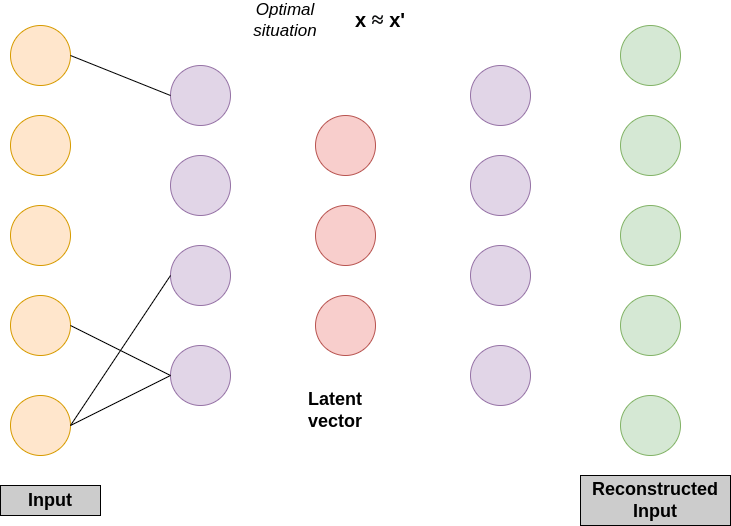
\includegraphics[scale=0.4]{figures/ae.png}
    \caption{Example of a dense autoencoder architecture}
    \label{fig:aediagram}
\end{figure}

The optima for any kind of autoencoder becomes that of lossless encoding, which can be described as such:

\begin{equation}
    X' = D_\theta(E_\phi(X))
\end{equation}

As mentioned in Section \ref{back:linear}, dense networks can struggle with feature extraction. This is also the case for dense autoencoders. By introducing convolutional layers, the autoencoder becomes more adept at image recognition tasks [CITE], signal analysis, and anomaly detection on these data types. These networks are called convolutional autoencoders (\acrshort{cae}).  \\

When the model is sufficiently trained for a specific task, $D$ \textit{may} become unnecessary for certain applications such as data reconstruction or denoising [CITE]. If the primary goal is feature extraction or dimensionality reduction, $E$ alone can be used to map input data to the lower-dimensional latent space. By utilizing only $E$, the overall complexity and size of the model $M$ can be reduced, which may be beneficial in scenarios with computational or memory constraints. For other tasks, such as autoencoders, include image reconstruction \cite{7797236}, signal analysis \cite{andrysiak2016machine}, and anomaly detection \cite{bank2021autoencoders}, the whole model is often needed.
\subsubsection{Latent Space}

The latent space $Z$ in autoencoders aims to capture essential features of the input data $X$ in a lower-dimensional representation. However, traditional autoencoders face limitations in their generative capabilities [CITE]. While they are trained to reconstruct original data accurately, they typically lack the ability to generate new, diverse samples from $Z$.
This limitation arises from the fact that regular autoencoders do not impose any specific structure on $Z$ beyond compressing the $X$. As a result, the latent representations may not be continuous or meaningful for interpolation and generation tasks.



\subsubsection{Loss functions for autoencoders}

The goal of an autoencoder is to make the reconstructed output $\hat{X}$ as close to the input $X$ as possible. Given this, the loss function used for these networks can be seen as a distance metric, where the objective is to minimize the distance $d$ between input and output:

\begin{equation}
    \mathcal{L}(\theta; X) = d(X, \hat{X}) = d(X, f_\theta(X))
\end{equation}
The optimization problem can then be formulated as:
\begin{equation}
    \theta^* = \argmin_{\theta} \mathbb{E}_{X \sim p_{\text{data}}(X)}[\mathcal{L}(\theta; X)]
\end{equation}
where $\theta^*$ are the optimal parameters for the network. Some of the more common loss functions used for autoencoders includes: \\

\clearpage
\textbf{\acrfull{mse}}

\begin{equation}\label{eq:mse}
    \mathcal{L}_{\text{MSE}}(x, \hat{x}) = \dfrac{1}{N}  \sum_{i=1}^{N}(x_i-\hat{x}_i)^2
\end{equation}

The \acrshort{mse} loss function is a commonly used loss function. It punishes bigger differences by squaring the difference between two elements in the prior $x$ and the posterior $\hat{x}$. It then outputs the mean of all the squarred errors computed. \\

\textbf{\acrfull{mae}}

\begin{equation}\label{eq:mae}
    \mathcal{L}_{\text{MAE}}(x, \hat{x}) = \dfrac{1}{N}  \sum_{i=1}^{N}|x_i-\hat{x}_i|
\end{equation}

The \acrshort{mae} loss function is quite similar to the \acrshort{mse} function. The difference is that the \acrshort{mae} function returns the absolute value of the distance between two distributions $x$ and $\hat{x}$, thus equally punishing all errors. \\

In addition to the issues with regular autoencoders in regards to decoding the latent space, these autoencoders have several disadvantages, including:

\begin{itemize}
    \item \textbf{Overfitting}: If the encoder and decoder become too powerful, they can learn to simply copy the input data to the output data.
    \item \textbf{Lack of regularization}: This can lead to poor generalization to unseen data
    \item \textbf{Input sensitivity}: Noise in the input data may potentially lead to large changes in the latent space
    \item \textbf{Interpretability}: The latent space may not be interpretable or correspond to meaningful features of the data
    \item \textbf{Encoding determinism}: Regular autoencoders don't account for uncertainty or multiple plausible interpretations of the input.
\end{itemize}